% ---------------------------------------------------------------- 34
% [suite]
\begin{frame}{Diagnostics : la liste de contrôle à passer en revue}
% [rogna]
\footnotesize
\begin{center}
\footnotesize
\begin{tabular}{@{}p{3.0cm}p{3.4cm}p{3.0cm}p{4.2cm}@{}}
\toprule
\textbf{Diagnostic} & \textbf{Ce qu'il détecte} & \textbf{Seuil d'alerte} & \textbf{Commande PyMC / ArviZ} \\
\midrule
Trace plot & non-stationnarité, sauts, tendance & visuelle & \py{az.plot_trace(idata)} \\[1.5mm]
Rank plot & modes non visités, chaînes divergentes & non uniforme & \py{az.plot_rank(idata)} \\[1.5mm]
$\hat R$ (R-hat) & désaccord entre et dans les chaînes & $> 1{,}01$ & \py{az.rhat(idata)} \\[1.5mm]
ESS (bulk / tail) & autocorrélation, queues mal explorées & $< 400$ \; (\;proche de 100 : alerte) & \py{az.ess(idata)} \\[1.5mm]
Divergences & géométrie pathologique & $> 0$ & \py{idata.sample\_stats.diverging} \\[1.5mm]
MCSE & erreur de simulation sur la moyenne & comparer à l'effet cherché & \py{az.mcse(idata)} \\[1.5mm]
PPC & modèle inadéquat (pas l'échantillonneur) & couverture $\ne$ 94 \% & \py{az.plot\_ppc(idata)} \\
\bottomrule
\end{tabular}
\end{center}
\vspace{1mm}
\end{frame}

% [suite]
\begin{frame}{Diagnostics : la liste de contrôle à passer en revue (suite)}
\begin{columns}[t]
\begin{column}{0.49\textwidth}
\begin{kbox}[La règle des quatre questions]
\begin{enumerate}
  \item La chaîne a-t-elle \textbf{oublié} son départ ? (trace, burn-in)
  \item Les chaînes \textbf{racontent-elles la même histoire} ? ($\hat R$, rank)
  \item Y a-t-il assez de tirages \textbf{utiles} ? (ESS, MCSE)
  \item Le modèle est-il \textbf{adéquat} ? (PPC) --- question distincte des trois
        premières : un échantillonneur parfait peut valider un mauvais modèle.
\end{enumerate}
\end{kbox}
\end{column}
\begin{column}{0.49\textwidth}
\begin{wbox}[Deux confusions à ne plus faire]
\nok{} Confondre \textbf{convergence de la chaîne} et \textbf{qualité du modèle} :
les diagnostics ne jugent que le premier point.
\\[1mm]
\nok{} Croire qu'un $\hat R$ parfait suffit : deux chaînes peuvent être d'accord
sur \emph{un} mode alors que la cible en compte deux.
\end{wbox}
\end{column}
\end{columns}
\end{frame}

% ---------------------------------------------------------------- 35
\begin{frame}{Anatomie d'un rapport de diagnostics (résultats PyMC réels)}
\begin{center}
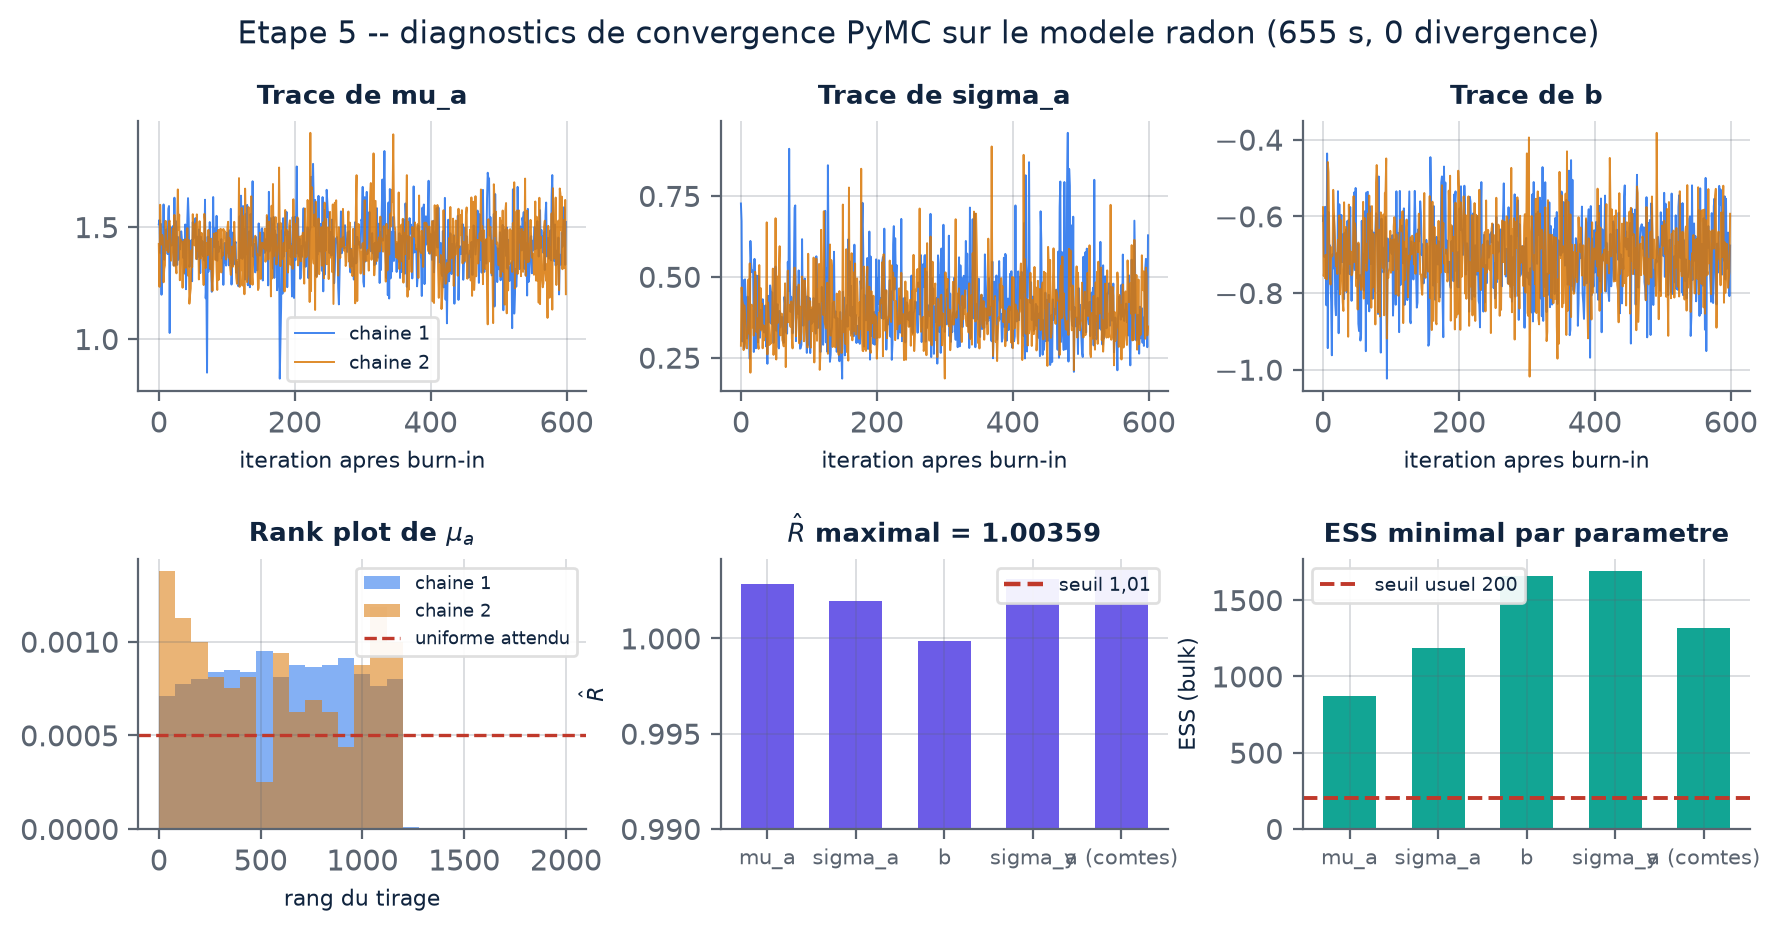
\includegraphics[width=0.90\textwidth]{j10_pymc_diagnostics.png}
\end{center}
\vspace{-1.5mm}
\centering\footnotesize
Modèle hiérarchique radon (section 5.5), 2 chaînes $\times$ 1 000 tirages après
1 000 de chauffe, \py{target\_accept=0.9}, \py{cores=1} :
$\hat R_{\max} = $ 1,00311 \;; \; ESS minimal = 872 \;; \;
divergences = 0 \;; \; temps d'échantillonnage 655~s.
\end{frame}

% ---------------------------------------------------------------- 36
\begin{frame}{Le trace plot : cinq pathologies à reconnaître}
% [rogna]
\small
\begin{columns}[t]
\begin{column}{0.53\textwidth}
\begin{ebox}[Ce qu'on regarde]
\begin{enumerate}
  \item Deux chaînes qui \textbf{ne se recouvrent pas} : \;
        $\hat R$ explose, rien n'est stationnaire.
  \item Une \textbf{tendance} qui persiste après le burn-in : \;
        la chauffe était trop courte (ou la chaîne se déplace lentement).
  \item De \textbf{longs paliers} : \;
        proposition trop large --- ESS effondré (mesuré : ESS = 130 à $s = 6$).
  \item Une trace \textbf{trop lisse}, sans bruit : \;
        proposition trop étroite --- ESS = 46 à $s = 0{,}02$.
  \item Une chaîne \textbf{plate} à une valeur : \;
        le paramètre n'est pas identifié par les données, ou le prior est écrasant.
\end{enumerate}
\end{ebox}
\end{column}
\begin{column}{0.45\textwidth}
\begin{kbox}[Comment le lire efficacement]
\begin{itemize}
  \item Toujours \textbf{superposer} les chaînes d'une même couleur.
  \item Ne pas juger sur 100 itérations : afficher au moins 500 à 1 000 tirages
        par chaîne.
  \item La trace est un diagnostic \emph{qualitatif} : elle \emph{complète}
        $\hat R$ et l'ESS, elle ne les remplace pas.
  \item Sur 200 paramètres \emph{on ne regarde pas} les 200 traces : on regarde
        les 5 paramètres d'intérêt et les cas signalés par $\hat R$.
\end{itemize}
\end{kbox}
\begin{tcolorbox}[colback=byCyan!8,colframe=byCyan,arc=2mm]
\small\textbf{Réflexe :} une trace saine ressemble à du \emph{bruit autour d'un
niveau stable}, sans structure visible.
\end{tcolorbox}
\end{column}
\end{columns}
\end{frame}

% ---------------------------------------------------------------- 37
% [suite]
\begin{frame}{Rank plot : voir ce que le trace plot cache}
\begin{columns}[t]
\begin{column}{0.52\textwidth}
\begin{ebox}[Construction]
Pour un paramètre et ses $K$ chaînes :
\begin{enumerate}
  \item empiler tous les tirages de toutes les chaînes ;
  \item remplacer chaque tirage par son \textbf{rang} dans cet ensemble ;
  \item histogrammer les rangs \emph{séparément par chaîne}.
\end{enumerate}
Si les chaînes ont convergé, chaque histogramme est \textbf{uniforme} sur
$[0, KN]$ : aucune chaîne ne concentre les grandes ou les petites valeurs.
\end{ebox}
\end{column}
\begin{column}{0.46\textwidth}
\begin{kbox}[Les deux motifs pathologiques]
\begin{itemize}
  \item \textbf{Rangs groupés à une extrémité} pour une chaîne : elle est restée
        dans une région de faible densité $\Rightarrow$ mode non visité,
        initialisation mal placée.
  \item \textbf{Forme en U} (les extrêmes sur-représentés) : les queues sont mal
        échantillonnées $\Rightarrow$ intervalles de crédibilité trop étroits :
        exactement le risque qu'on cherche à éviter.
\end{itemize}
\end{kbox}
\end{column}
\end{columns}
\end{frame}

% [suite]
\begin{frame}{Rank plot : voir ce que le trace plot cache (suite)}
\begin{solbox}[Sur nos chaînes radon]
Les rangs des deux chaînes sont uniformes : le trace plot \emph{et} le rank plot
concordent. Quand les deux se contredisent, c'est le rank plot qui a raison sur
la question des modes multiples.
\end{solbox}

\end{frame}

% ---------------------------------------------------------------- 38
\begin{frame}{R-hat : le désaccord entre et dans les chaînes}
% [rogna]
\footnotesize
\begin{columns}[t]
\begin{column}{0.53\textwidth}
\begin{ebox}[Définition opérationnelle]
Avec $m$ chaînes de longueur $n$ :
\[
\hat R = \sqrt{\frac{\hat V}{W}}, \qquad
W = \text{variance intra-chaîne},
\]
et $\hat V$ combine $W$ et la variance \textbf{entre} les moyennes de chaînes.
\\[1mm]
Intuition : si les chaînes ont oublié leur point de départ, la variabilité
\emph{entre} chaînes est du même ordre que la variabilité \emph{dans} une chaîne,
donc $\hat R \to 1$ par le haut.
\end{ebox}
\begin{kbox}[Le seuil de 1,01, et pourquoi il est si strict]
Un $\hat R$ de 1,1 peut cacher des intervalles de crédibilité sous-estimés de
30 \% : l'échelle est en $\sqrt{\cdot}$, donc 1,01 en $\hat R$ signifie déjà un
écart de 2 \% sur les variances. En 2026 on rapporte le \emph{maximum} de
$\hat R$ sur \emph{tous} les paramètres, y compris les effets de groupe.
\end{kbox}
\end{column}
\begin{column}{0.45\textwidth}
\begin{solbox}[Mesures de la section 5.5 (modèle radon)]
\footnotesize\begin{tabular}{@{}p{4.3cm}p{1.6cm}@{}}
\toprule
paramètre & $\hat R$ \\
\midrule
maximum sur $\mu_a$, $\sigma_a$, $b$, $\sigma_y$ & 1,00311 \\
maximum sur les 12 intercepts $a_j$ & 1,00359 \\
\midrule
$\hat R_{\max}$ global & \textbf{1,00311} \\
\bottomrule
\end{tabular}
\vspace{1.5mm}
\\ Le seuil de 1,01 est respecté partout : on peut lire les intervalles de crédibilité.
\end{solbox}
\begin{wbox}[Et si $\hat R$ vaut 1,00 avec 50 tirages ?]
Un $\hat R$ parfait ne prouve rien si l'ESS vaut 3. \;\textbf{Toujours} lire
$\hat R$ \emph{et} ESS ensemble : ce sont deux pathologies différentes.
\end{wbox}
\end{column}
\end{columns}
\end{frame}

% ---------------------------------------------------------------- 39
\begin{frame}{ESS : combien de tirages utiles ai-je vraiment ?}
% [rogna]
\small
\begin{columns}[t]
\begin{column}{0.5\textwidth}
\begin{ebox}[Rappels et seuils de travail]
\[
\mathrm{ESS} = \frac{N}{1 + 2\sum_{k \ge 1}\rho_k},
\qquad
\text{MCSE} = \frac{\hat\sigma}{\sqrt{\mathrm{ESS}}} .
\]
Repères utilisés en pratique :
\begin{itemize}
  \item $\mathrm{ESS} > 400$ : suffisant pour une moyenne et un écart-type stables.
  \item $\mathrm{ESS} > 100$ \emph{par queue} pour un quantile extrême
        (ArviZ distingue \py{bulk} et \py{tail}).
  \item $\mathrm{ESS} < 100$ : les intervalles changent d'une exécution à l'autre.
  \item Toujours comparer l'ESS au budget \textbf{par paramètre}, pas global.
\end{itemize}
\end{ebox}
\end{column}
\begin{column}{0.48\textwidth}
\begin{solbox}[ESS par itération, mesuré dans ce chapitre]
\scriptsize\begin{tabular}{@{}p{2.4cm}p{1.8cm}p{1.8cm}@{}}
\toprule
échantillonneur & cible & ESS / itération \\
\midrule
Monte-Carlo i.i.d. & Beta$(2,5)$ & 1,000 \\
MH $s$ = 0,35 & Beta$(2{,}5;7)$ & 0,197 \\
MH $s$ = 1,2 & $\N_2$, $\rho$ = 0,85 & 0,043 \\
Gibbs & $\N_2$, $\rho$ = 0,85 & 0,167 \\
HMC $\varepsilon$ = 0,30, $L$ = 10 & $\N_2$, $\rho$ = 0,95 & 1,000 \\
NUTS & $\N_2$, $\rho$ = 0,95 & 0,162 \\
PyMC NUTS & radon $a_j$ (le pire) & 1 315 / 1 200 \\
\bottomrule
\end{tabular}
\end{solbox}
\begin{kbox}[Le vrai critère : ESS par seconde ou par évaluation]
Sur la cible $\N_2$, HMC atteint l'ESS 1,000 par itération mais paie 10 évaluations
de gradient : $0{,}10$ ESS par évaluation, contre $0{,}197$ pour un MH d'une seule
évaluation. C'est le \emph{budget} qui tranche, pas l'ESS seul.
\end{kbox}
\end{column}
\end{columns}
\end{frame}

% ---------------------------------------------------------------- 40
% [suite]
\begin{frame}{Pourquoi plusieurs chaînes, et comment les comparer}
\begin{columns}[t]
\begin{column}{0.49\textwidth}
\begin{ebox}[Le principe]
Une seule chaîne ne peut pas dire si elle a « oublié » son départ, ni si elle a
manqué un mode : elle n'a rien à quoi se comparer.
\\[1mm]
En démarrant $K$ chaînes de points \textbf{dispersés} (PyMC les initialise en
tirant dans le prior), on obtient :
\begin{itemize}
  \item un estimateur de la variance entre chaînes $\Rightarrow$ $\hat R$ ;
  \item un test visuel de recouvrement (traces superposées) ;
  \item un détecteur de multimodalité (rank plot) ;
  \item un moyen de vérifier la \textbf{reproductibilité} (graines différentes).
\end{itemize}
\end{ebox}
\end{column}
\begin{column}{0.49\textwidth}
\begin{kbox}[Combien, et combien de temps ?]
\begin{itemize}
  \item Minimum utile : \textbf{2} chaînes ($\hat R$ est mal estimé avec 1).
  \item Recommandation ArviZ / Stan : \textbf{4 chaînes}, souvent suffisantes.
  \item Longueur : si $\hat R = 1{,}05$ avec 1 000 tirages, il faut environ
        $5 \times 1\,000$ tirages supplémentaires pour espérer passer sous
        1,01 --- \emph{et} une correction de la géométrie.
  \item Contrainte matérielle réelle sur cette machine (pas de compilateur C) :
        2 chaînes, 1 000 tirages, \py{cores=1}. On le déclare, et on vérifie
        que l'ESS reste suffisant.
\end{itemize}
\end{kbox}
\end{column}
\end{columns}
\end{frame}

% [suite]
\begin{frame}{Pourquoi plusieurs chaînes, et comment les comparer (suite)}
\begin{solbox}[Ce que cela change concrètement]
Avec 2 chaînes $\times$ 1 000 tirages sur le modèle radon :
$\hat R_{\max}$ = 1,00311 et ESS minimal = 872.
Avec 1 seule chaîne, aucune de ces deux vérifications n'existerait.
\end{solbox}

\end{frame}

% ---------------------------------------------------------------- 41
% [rogna]
% [rogna]
% [rogna]
% [split]
\begin{frame}{Contrôle prédictif a posteriori : le modèle tient-il ses promesses ?}
\begin{center}
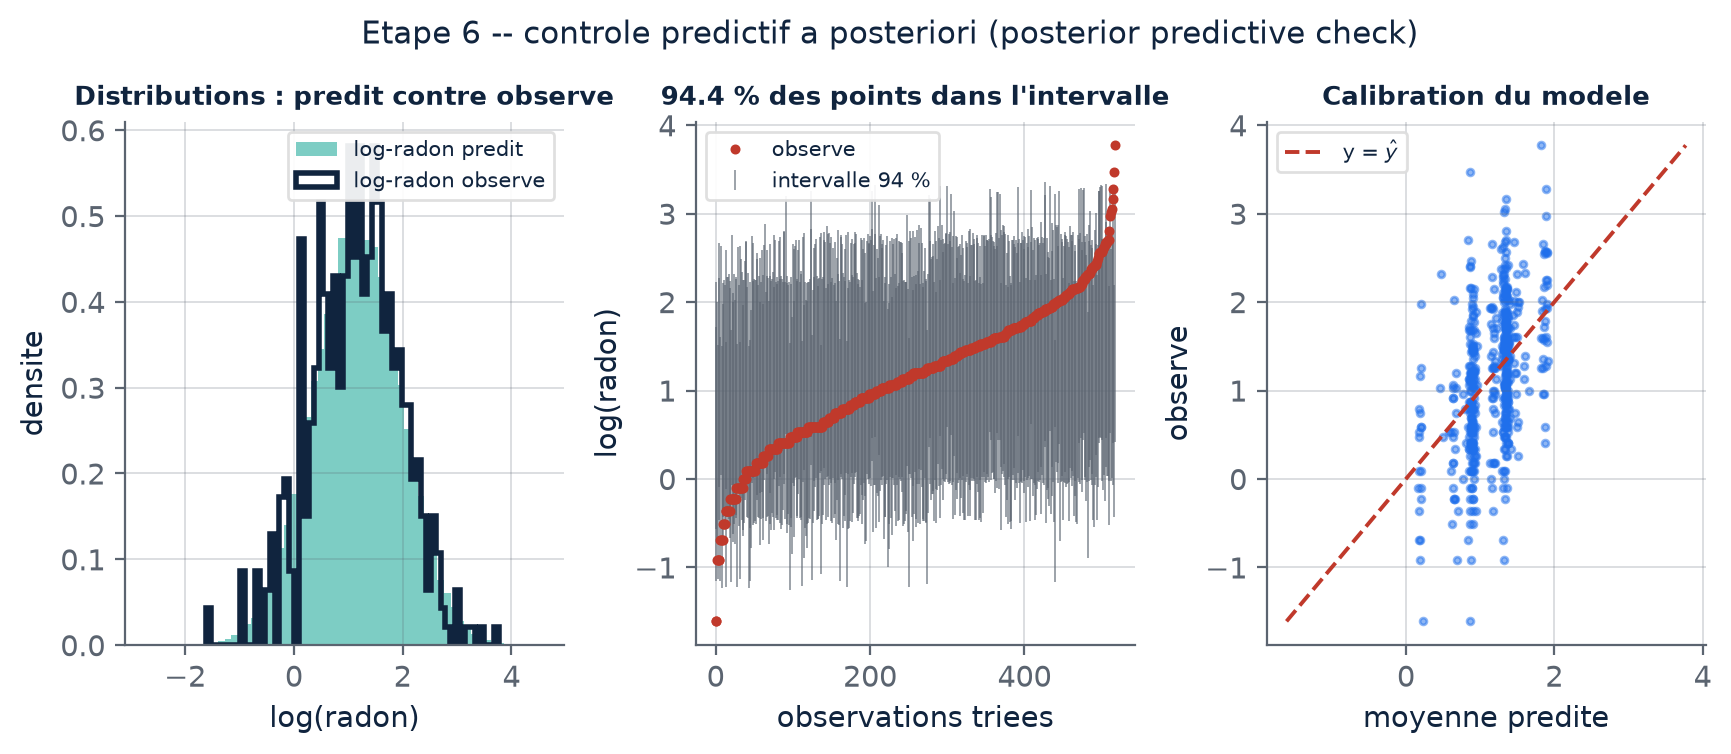
\includegraphics[width=.86\textwidth]{j11_ppc_radon.png}
\end{center}
\end{frame}

% [split]
\begin{frame}{Contrôle prédictif a posteriori : le modèle tient-il ses promesses ?}

\vspace{-1.5mm}
\begin{columns}[t]
\begin{column}{0.5\textwidth}
\begin{solbox}[Procédure et mesures (modèle radon, 1 200 tirages)]
\begin{enumerate}
  \item tirer $\tilde y^{(i)} \sim p(\tilde y \given \theta^{(i)})$ pour chaque
        tirage du posterior (2 000 réplications ici) ;
  \item comparer les \textbf{distributions} de $\tilde y$ et de $y$ ;
  \item compter la proportion d'observations couvertes par l'intervalle 94 \%.
\end{enumerate}
Mesures : couverture 94,4 \% ; moyenne observée 1,156 contre
1,156 prédite ; écart-type observé 0,805 contre
0,811 prédit.
\end{solbox}
\end{column}
\begin{column}{0.48\textwidth}
\begin{kbox}[Ce qu'un PPC révèle (et ne révèle pas)]
\begin{itemize}
  \item Il teste le \textbf{modèle} : forme de la vraisemblance, priors, effets
        oubliés. Un PPC raté n'est \emph{pas} un problème d'échantillonnage.
  \item Ici la couverture est proche du nominal et les moyennes coïncident :
        le log-radon par comté est raisonnablement décrit.
  \item Un excès de valeurs extrêmes observées signalerait des queues trop
        légères (passer à une Student, ou modéliser la surdispersion).
  \item Le PPC ne « prouve » pas que le modèle est vrai : il ne détecte que les
        incohérences qu'on a pensé à regarder.
\end{itemize}
\end{kbox}
\end{column}
\end{columns}
\end{frame}

% ---------------------------------------------------------------- 42
% [split]
\begin{frame}{Valider la chaîne contre une référence exacte}
\begin{center}
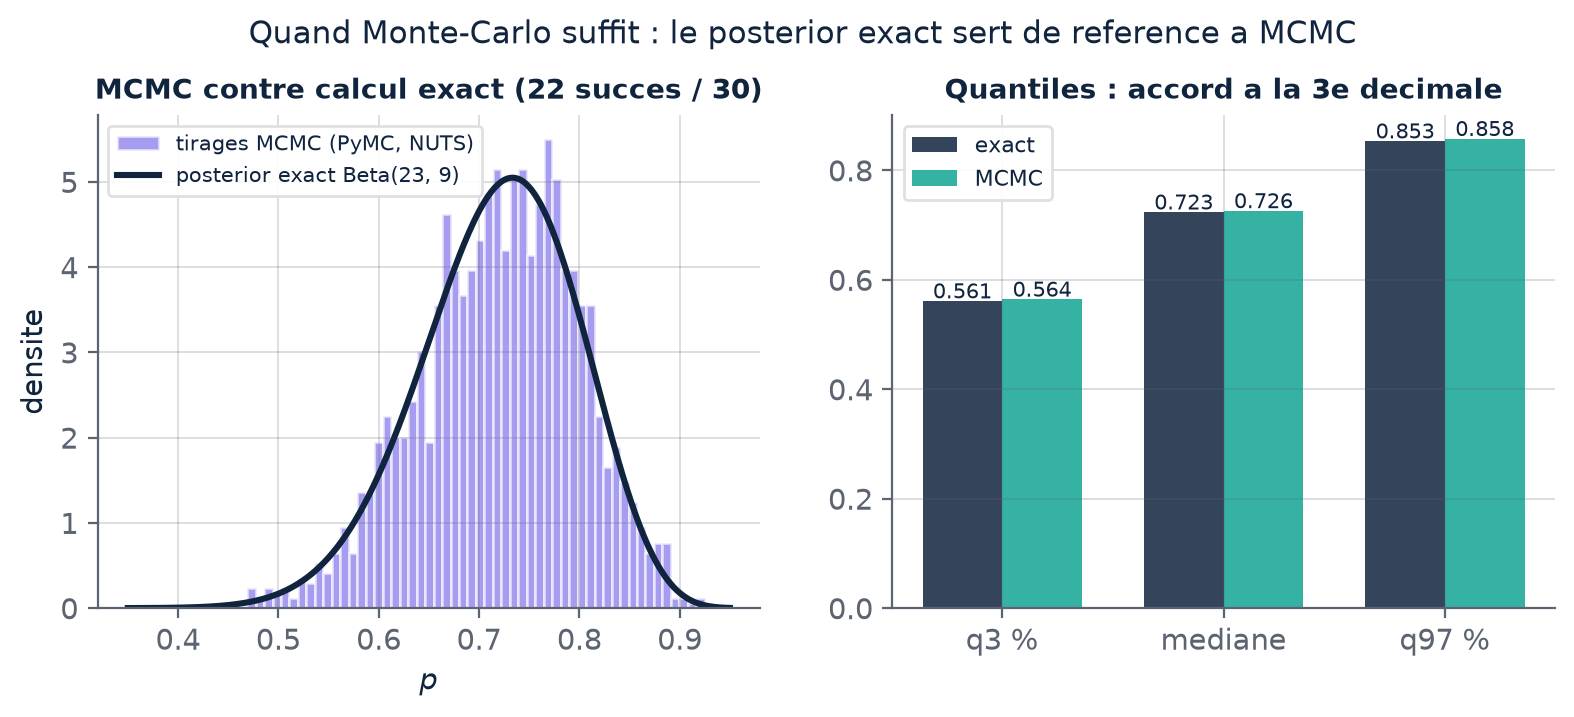
\includegraphics[width=\textwidth]{j14_mcmc_vs_exact.png}
\end{center}
\end{frame}

% [split]
% [suite5]
\begin{frame}{Valider la chaîne contre une référence exacte}
% [rogna]
\small
\begin{columns}[t]
\begin{column}{0.46\textwidth}
\begin{ebox}[Le test le plus simple qui vaut la peine]
On se place dans un cas où le posterior est \textbf{connu} : prior Beta$(1,1)$,
vues Binomiales, $k$ = 22 succès sur $n$ = 30 essais $\Rightarrow$
$p \given \data \sim \mathrm{Beta}(23, 9)$, donc
$\E[p \given \data] = 23/32 = 0{,}71875$.
\end{ebox}
\end{column}
\end{columns}
\end{frame}

% [suite5]
\begin{frame}{Valider la chaîne contre une référence exacte (suite)}
\begin{solbox}[Accord mesuré]
\footnotesize\begin{tabular}{@{}p{1.7cm}p{1.5cm}p{1.8cm}@{}}
\toprule
quantité & exact & MCMC (PyMC) \\
\midrule
moyenne & 0,71875 & 0,72067 \\
$q_{3\,\%}$ & 0,5610 & 0,5641 \\
médiane & 0,7234 & 0,7258 \\
$q_{97\,\%}$ & 0,8533 & 0,8576 \\
\midrule
$\hat R$ & --- & 1,00592 \\
ESS & --- & 593,7 \\
\bottomrule
\end{tabular}
\vspace{1mm}
\\ Écart absolu sur la moyenne : \textbf{0,00192}. La chaîne est donc
correcte ; tout écart restant est l'erreur de simulation elle-m\^eme.
\end{solbox}
\end{frame}

% ---------------------------------------------------------------- 43
\begin{frame}{Que faire quand ça ne converge pas : procédure ordonnée}
% [rogna]
\footnotesize
\begin{columns}[t]
\begin{column}{0.52\textwidth}
\begin{abox}[Procédure (dans cet ordre)]
\begin{enumerate}
  \item \textbf{Lire les avertissements} de PyMC mot à mot : ils nomment le
        problème (« 14 divergences after tuning », « ESS is extremely low »).
  \item \textbf{Contrôler les divergences} : si $> 0$, ne rien interpréter
        avant de les avoir supprimées.
  \item \textbf{Reparamétrer} : centrée $\rightarrow$ non centrée, échelles des
        prédicteurs, paramètres à contraintes (log, logit).
  \item \textbf{Augmenter \py{target\_accept}} (0,9 $\rightarrow$ 0,95
        $\rightarrow$ 0,99) : plus sûr, mais plus lent.
  \item \textbf{Allonger \py{tune}} et augmenter \py{init} (\py{"adapt\_diag"}) si
        le démarrage échoue.
  \item \textbf{Simplifier le modèle} : retirer un effet, remplacer une
        distribution, borner un prior.
  \item \textbf{Changer d'échantillonneur} en dernier recours : Gibbs si les
        conditionnelles sont closes, métropole à l'intérieur de Gibbs pour les
        variables discrètes.
\end{enumerate}
\end{abox}
\end{column}
\begin{column}{0.46\textwidth}
\begin{wbox}[Les trois erreurs qui font perdre une journée]
\nok{} \textbf{Augmenter les tirages} alors que le problème est géométrique :
le $\hat R$ ne bougera pas.\\[1mm]
\nok{} \textbf{Supprimer le burn-in} pour « nettoyer » un $\hat R$ élevé :
il ne mesure qu'après la chauffe, cela ne change rien.\\[1mm]
\nok{} \textbf{Thinner} pour faire baisser l'autocorrélation : l'ESS de ce qui
reste est identique, on a juste jeté des tirages.
\end{wbox}
\begin{kbox}[Le réflexe qui marche]
Dans 80 \% des cas de non-convergence sur un modèle hiérarchique, la cause est
l'écriture \emph{centrée} (slide 30) : passer en non centré fait tomber les
divergences de 17 à 0 et multiplie l'ESS par 8 sur notre exemple.
\end{kbox}
\end{column}
\end{columns}
\end{frame}

% ---------------------------------------------------------------- 44
\begin{frame}{Synthèse 5.4 --- Diagnostics et validation}
\begin{columns}[t]
\begin{column}{0.49\textwidth}
\begin{tcolorbox}[enhanced,colback=byPurple!7,colframe=byPurple,arc=2mm,
   title={\bfseries\color{white}\faLightbulb\ Synthèse},colbacktitle=byPurple,
   attach boxed title to top left={xshift=3mm,yshift=-2mm},
   boxed title style={arc=1mm,boxrule=0pt}]
\begin{itemize}
  \item \textbf{Trace} : qualitatif, détecte la non-stationnarité. À regarder en
        premier, à ne jamais confondre avec une preuve.
  \item \textbf{Rank plot} : le seul outil visuel qui voit un mode manqué.
  \item \textbf{$\hat R < 1{,}01$} sur \emph{tous} les paramètres : mesuré à
        1,00311 sur le modèle radon.
  \item \textbf{ESS} : le nombre de tirages utiles ; sous 100, aucun intervalle
        n'est fiable. À comparer au coût (ESS par évaluation de gradient).
  \item \textbf{Divergences} : zéro, ou rien d'autre. Mesuré : 17 en paramétrisation
        centrée, 0 en non centrée.
  \item \textbf{PPC} : valide le \emph{modèle}, pas la chaîne --- et c'est une
        étape obligatoire avant toute décision.
  \item \textbf{Validation} : quand un posterior exact existe, comparer (accord
        à la 3\ieme{} décimale obtenu ici).
\end{itemize}
\end{tcolorbox}
\end{column}
\begin{column}{0.49\textwidth}
\begin{qbox}[Quiz de diagnostic -- que concluez-vous ?]
\textbf{Cas A.} $\hat R$ = 1,004 ; ESS = 38 pour $b$ ; 0 divergence.
\\ \footnotesize Convergence apparente mais précision insuffisante : allonger la
chaîne ou améliorer la géométrie.\\[1.5mm]
\textbf{Cas B.} $\hat R = 1{,}00$ ; ESS = 1 200 ; 3 divergences sur 4 000.
\\ \footnotesize Le plus dangereux : tout semble parfait, mais 3 zones du
posterior n'ont pas été explorées. Reparamétrer et relancer.\\[1.5mm]
\textbf{Cas C.} Tous les diagnostics sont parfaits, mais le PPC donne une
couverture de 71 \% pour un intervalle annoncé à 94 \%.
\\ \footnotesize La chaîne est bonne, le \emph{modèle} est faux : ajouter un effet
ou changer la vraisemblance.\\[1.5mm]
\textbf{Cas D.} Les deux chaînes donnent $\bar\theta$ = 0,31 et 0,72, $\hat R$ = 2,4.
\\ \footnotesize Deux modes, chaînes initialisées de part et d'autre : la multimodalité
doit être traitée dans le modèle (ou par échantillonnage par tempérage), pas par
plus de tirages.
\end{qbox}
\end{column}
\end{columns}
\end{frame}

% ---------------------------------------------------------------- 45
\begin{frame}{Mini-projet guidé : le radon du Minnesota (section 5.5)}
% [rogna]
\small
\begin{columns}[t]
\begin{column}{0.52\textwidth}
\begin{ebox}[Les données, et la question posée]
Fichier \file{src/data/srrs2.dat} (10\,000 lignes d'origine, 919 mesures du
Minnesota). On retient les \textbf{12 comtés les plus mesurés} :
\begin{itemize}
  \item 518 mesures, 12 comtés ;
  \item 65 logements au premier étage, 453 en sous-sol ;
  \item concentration en radon : moyenne \textbf{1,1558} en log(pCi/L),
        écart-type 0,805 ;
  \item 7 \% des mesures dépassent 10 pCi/L, le seuil d'action
        de l'agence américaine (log(10) = 2,3026) ;
  \item moyenne brute : premier étage 0,606 contre sous-sol 1,235,
        soit une différence de -0,629 en log, c'est-à-dire
        $\exp(-0{,}629) = 0{,}53$.
\end{itemize}
\textbf{Question :} l'effet « premier étage » est-il réel et de quelle taille,
comté par comté ?
\end{ebox}
\end{column}
\begin{column}{0.46\textwidth}
\begin{abox}[Grille d'évaluation notée (20 points)]
\footnotesize\begin{tabular}{@{}p{4.8cm}r@{}}
\toprule
étape & points \\
\midrule
1. Formulation probabiliste complète, variables et indices & 2 \\
2. Justification des priors (échelle, ordre de grandeur) & 3 \\
3. Vérification prédictive \emph{a priori} et critique du prior & 2 \\
4. Échantillonnage reproductible (graines, taille, réglages) & 3 \\
5. Diagnostics \emph{complets} et interprétés (trace, $\hat R$, ESS, divergences) & 5 \\
6. Contrôle prédictif \emph{a posteriori} & 2 \\
7. Décision chiffrée avec intervalle et restitution écrite & 3 \\
\midrule
total & 20 \\
\bottomrule
\end{tabular}
\vspace{1mm}
\\
\footnotesize Les points 5 et 2 sont les plus discriminants : un modèle qui
« tourne » sans diagnostics interprétés ne vaut pas la moitié du barème.
\end{abox}
\end{column}
\end{columns}
\end{frame}

% ---------------------------------------------------------------- 46
% [split]
\begin{frame}{Étapes 1 à 3 : formulation, priors et vérification \emph{a priori}}
\begin{center}
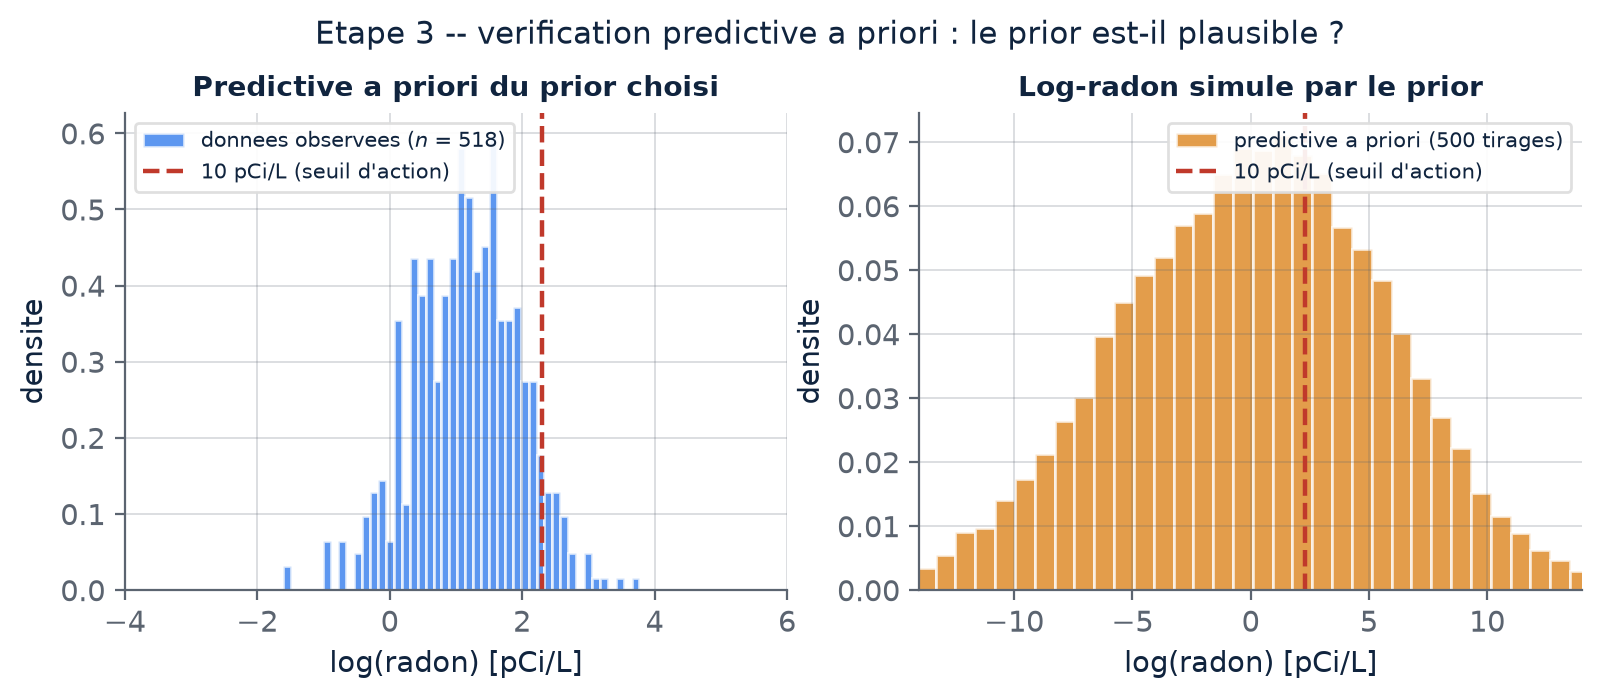
\includegraphics[width=\textwidth]{j13_prior_predictive.png}
\end{center}
\end{frame}

% [split]
% [suite]
\begin{frame}{Étapes 1 à 3 : formulation, priors et vérification \emph{a priori}}
% [rogna]
\footnotesize
\begin{columns}[t]
\begin{column}{0.52\textwidth}
\begin{ebox}[Étape 1 --- le modèle]
Notations : $y_{ij}$ = log-radon du logement $i$ du comté $j$ ;
$x_{ij} = 1$ si premier étage, $0$ sinon.
\[
y_{ij} \given a_j, b, \sigma_y \sim \N\!\big(a_j + b\,x_{ij},\; \sigma_y^2\big),
\qquad
a_j \given \mu_a, \sigma_a \sim \N(\mu_a, \sigma_a^2).
\]
Trois niveaux d'incertitude : le bruit $\sigma_y$, les écarts de comtés
$\sigma_a$, la moyenne générale $\mu_a$. C'est le modèle de Gelman--Hill
simplifié, et c'est un \textbf{modèle hiérarchique} : les comtés empruntent de
l'information à l'ensemble.
\end{ebox}
\end{column}
\begin{column}{0.46\textwidth}

\vspace{-2mm}
\begin{solbox}[Étape 3 — critique du prior]
500 simulations du prior : les log-radon simulés couvrent une plage
\emph{beaucoup plus large} que les données (de -13,34 à 13,25 aux
quantiles 1--99 \%), et 35,9 \% des valeurs simulées dépasseraient
10 pCi/L alors que les données sont à 7 \%.
\\[1mm]
Aucun prior n'exclut les données observées : ils sont \textbf{faiblement
informatifs mais pas absurdes}. Une telle vérification aurait invalidé un prior
comme $\N(0, 0{,}1)$ sur $\mu_a$.
\end{solbox}
\end{column}
\end{columns}
\end{frame}

% [suite]
\begin{frame}{Étapes 1 à 3 : formulation, priors et vérification \emph{a priori} (suite)}
\begin{kbox}[Étape 2 --- les priors, et pourquoi]
\footnotesize\begin{tabular}{@{}p{1.2cm}p{1.7cm}p{2.8cm}@{}}
\toprule
paramètre & prior & justification \\
\midrule
$\mu_a$ & $\N(0, 5)$ & log-radon plausible entre $-15$ et $+15$ \\
$\sigma_a$ & HalfNormal$(2)$ & dispersion inter-comtés de l'ordre de 1-2 \\
$b$ & $\N(0, 3)$ & effet d'étage plausible, large mais borné \\
$\sigma_y$ & HalfNormal$(2)$ & bruit résiduel de l'ordre de 1 \\
\bottomrule
\end{tabular}
\end{kbox}
\end{frame}

% ---------------------------------------------------------------- 47
\begin{frame}[fragile]{Étape 4 : l'échantillonnage, en quinze lignes}
\begin{columns}[t]
\begin{column}{0.55\textwidth}
\begin{codebox}[modele\_radon.py --- exécuté (PyMC 5.28, NUTS, 2 chaînes)]
\begin{lstlisting}[basicstyle=\ttfamily\fontsize{5.8}{6.6}\selectfont]
import pymc as pm, arviz as az
with pm.Model() as modele:
    mu_a    = pm.Normal("mu_a", 0.0, 5.0)
    sigma_a = pm.HalfNormal("sigma_a", 2.0)
    b       = pm.Normal("b", 0.0, 3.0)
    a       = pm.Normal("a", mu_a, sigma_a, shape=12)
    sigma_y = pm.HalfNormal("sigma_y", 2.0)
    pm.Normal("y", mu=a[idx] + b * x, sigma=sigma_y, observed=y)

    idata = pm.sample(draws=1000, tune=1000, chains=2,
                      cores=1, target_accept=0.9,
                      random_seed=7, progressbar=False)
    pm.sample_posterior_predictive(
        idata, extend_inferencedata=True)
\end{lstlisting}
\end{codebox}
\end{column}
\begin{column}{0.43\textwidth}
\begin{solbox}[Ce que produit cette exécution]
\footnotesize\begin{tabular}{@{}p{3.4cm}p{1.9cm}@{}}
\toprule
& mesure \\
\midrule
durée totale & 655 s \\
tirages (hors chauffe) & 1 200 ($2 \times 600$) \\
pas de NUTS au total & 8 520 \\
acceptation moyenne & 0,903 \\
divergences & 0 \\
$\hat R_{\max}$ & 1,00311 \\
ESS minimal & 872 \\
\bottomrule
\end{tabular}
\vspace{1.5mm}
\\ Pas de compilateur C sur cette machine : PyTensor tourne en Python pur. D'où
le choix de \py{cores=1}, de 2 chaînes et de 1 000 tirages --- contrainte
matérielle \textbf{déclarée} dans le rapport, pas dissimulée.
\end{solbox}
\end{column}
\end{columns}
\end{frame}

% ---------------------------------------------------------------- 48
\begin{frame}{Étape 5 : diagnostics du modèle radon, chiffre par chiffre}
% [rogna]
\small
\begin{center}
\footnotesize
\begin{tabular}{@{}p{2.9cm}p{2.2cm}p{2.2cm}p{4.9cm}@{}}
\toprule
\textbf{Paramètre} & \textbf{moyenne} & \textbf{IC 94 \%} & \textbf{Lecture} \\
\midrule
$\mu_a$ (moyenne des comtés) & 1,417 & [1,189 ; 1,668] &
log-radon moyen d'un sous-sol, toutes régions confondues \\[1.5mm]
$\sigma_a$ (dispersion) & 0,405 & [0,252 ; 0,678] &
les comtés diffèrent, mais modérément \\[1.5mm]
$b$ (premier étage) & -0,700 & [-0,896 ; -0,520] &
facteur 0,50 : le premier étage divise le radon par 2 \\[1.5mm]
$a_j$ (12 comtés) & 0,882 à 1,889 & --- &
les extrêmes bruts sont ramenés vers la moyenne \\[1.5mm]
$\sigma_y$ (bruit) & 0,720 & --- &
variabilité entre logements d'un même comté \\
\bottomrule
\end{tabular}
\end{center}
\vspace{1mm}
\begin{columns}[t]
\begin{column}{0.5\textwidth}
\begin{kbox}[Ce que ces nombres racontent]
L'effet de l'étage vaut $b = $ -0,700 en log : les logements du premier étage
ont $\exp(-0,700) = 0,497$ fois la concentration d'un sous-sol, soit environ
moitié moins. L'intervalle [-0,896 ; -0,520] exclut clairement 0 : l'effet est réel.
La dispersion inter-comtés $\sigma_a$ = 0,405 est petite devant l'étendue
des moyennes \emph{brutes} des comtés.
\end{kbox}
\end{column}
\begin{column}{0.5\textwidth}
\begin{wbox}[Ce que ces nombres ne disent pas]
Il ne s'agit \textbf{pas} d'un effet causal : la variable « étage » est corrélée à
l'âge du b\^atiment, à la géologie et au type de construction, non mesurés ici.
Le modèle quantifie une association, avec son incertitude --- rien de plus.
\end{wbox}
\end{column}
\end{columns}
\end{frame}

% ---------------------------------------------------------------- 49
% [rogna]
% [rogna]
% [rogna]
% [split]
\begin{frame}{Étape 6 : prédiction, décision et restitution}
\begin{center}
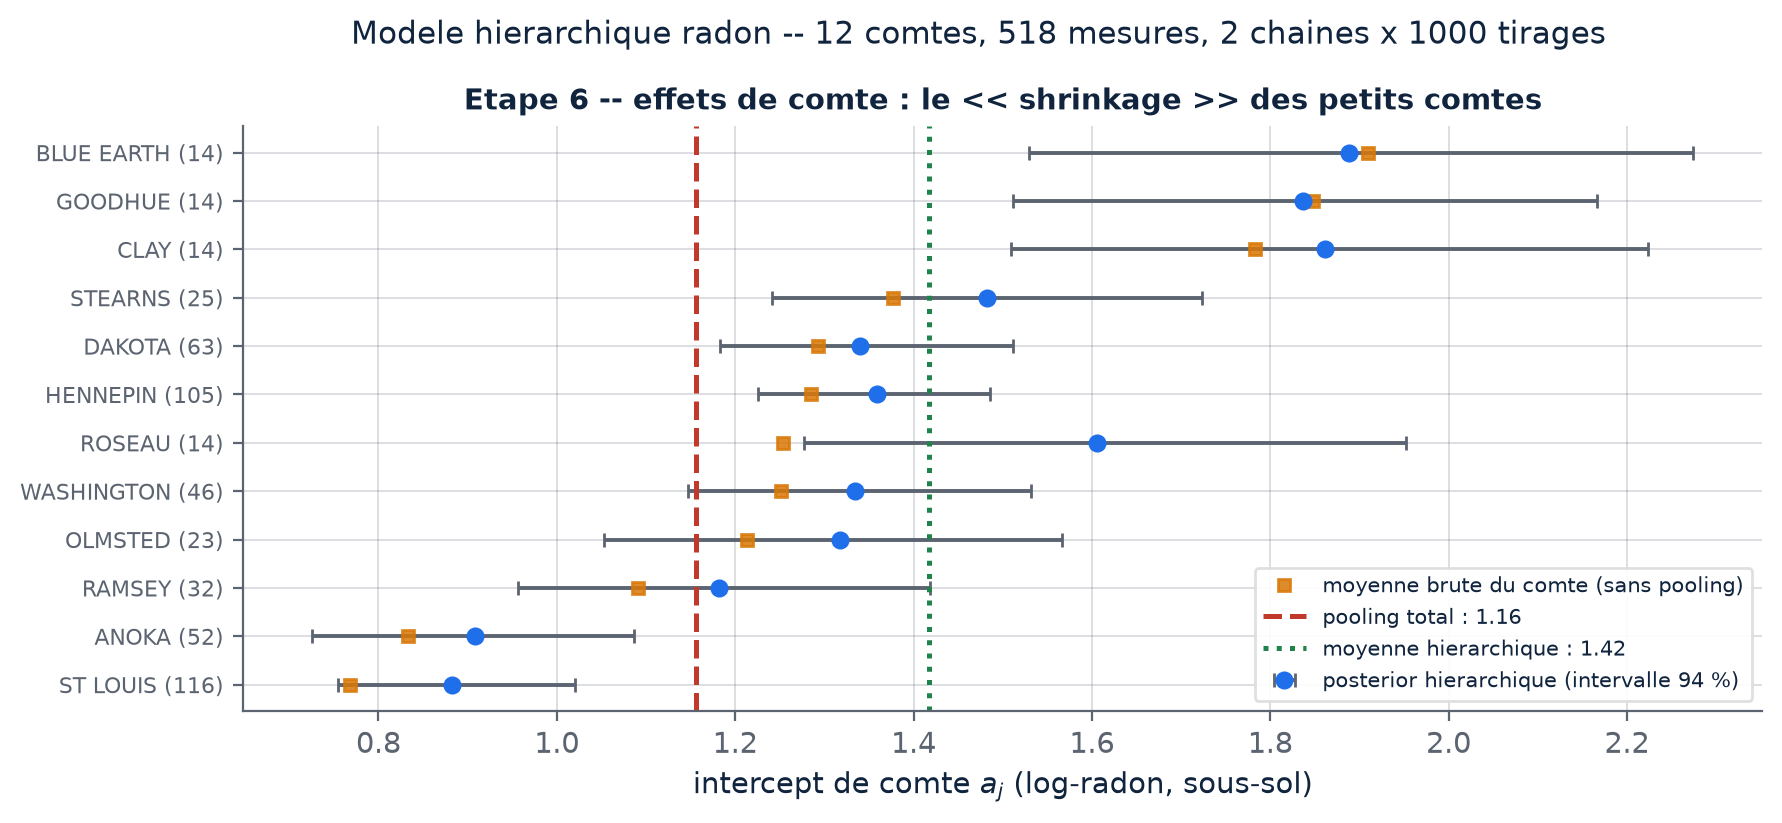
\includegraphics[width=.86\textwidth]{j12_forest_radon.png}
\end{center}
\end{frame}

% [split]
\begin{frame}{Étape 6 : prédiction, décision et restitution}

\vspace{-1.5mm}
\begin{columns}[t]
\begin{column}{0.52\textwidth}
\begin{solbox}[Le \emph{shrinkage}, mesuré]
\begin{itemize}
  \item Moyennes brutes : de 0,768 à 1,909 selon le comté.
  \item Après hiérarchie : de 0,882 à 1,889 : les comtés à
        petit effectif sont \textbf{ramenés vers la moyenne générale}
        (1,156).
  \item C'est ce qui rend le modèle hiérarchique supérieur à la comparaison de
        12 modèles séparés : chaque comté emprunte de la force aux autres.
\end{itemize}
\end{solbox}
\end{column}
\begin{column}{0.46\textwidth}
\begin{abox}[La décision qu'on ose écrire]
Avec $\hat b = $ -0,700 et un IC 94 \% de [-0,896 ; -0,520] :
\begin{quote}\small
« \textbf{Le premier étage divise la concentration médiane en radon par environ
2,0 par rapport à un sous-sol} (intervalle de crédibilité 94 \%
[1,68 ; 2,45]). Cette conclusion repose sur un modèle hiérarchique validé par ses
diagnostics ($\hat R_{\max}$ = 1,00311, 0 divergence) et par un contrôle
prédictif couvrant 94,4 \% des observations. »\end{quote}
C'est le format de restitution attendu au mini-projet : \textbf{un chiffre, un
intervalle, une phrase de portée}.
\end{abox}
\end{column}
\end{columns}
\end{frame}

% ---------------------------------------------------------------- 50
% [suite5]
\begin{frame}{Synthèse du chapitre 5 --- et ce que vous savez faire maintenant}
\begin{columns}[t]
\begin{column}{0.52\textwidth}
\begin{tcolorbox}[enhanced,colback=byPurple!7,colframe=byPurple,arc=2mm,
   title={\bfseries\color{white}\faLightbulb\ Les huit idées du chapitre},
   colbacktitle=byPurple,
   attach boxed title to top left={xshift=3mm,yshift=-2mm},
   boxed title style={arc=1mm,boxrule=0pt}]
\begin{enumerate}
  \item On ne calcule plus l'intégrale de Bayes : on la \textbf{simule}
        (erreur en $1/\sqrt N$, mesurée à la pente $-0{,}501$).
  \item Un noyau de transition invariant pour $\pi$ suffit à échantillonner :
        \textbf{bilan détaillé}.
  \item Metropolis-Hastings accepte avec $\min(1, \text{rapport})$ : la constante
        de normalisation disparaît.
  \item La proposition est le seul curseur (ESS optimal mesuré à $s$ = 0,35) et
        les tirages restent \textbf{corrélés} (ESS = 5 896 sur 30 000).
  \item Gibbs est exact et sans réglage, HMC utilise le gradient, NUTS choisit
        la longueur : ESS/\,itér.\ mesurés 0,167 / 1,000 / 0,162.
  \item Les \textbf{divergences} sont le symptôme de la mauvaise géométrie :
        17 en centré, 0 en non centré.
  \item \textbf{Trace, rank plot, $\hat R < 1{,}01$, ESS $> 400$, 0 divergence} :
        la liste de contrôle minimale.
  \item Le \textbf{PPC} valide le modèle, pas l'échantillonneur.
\end{enumerate}
\end{tcolorbox}
\end{column}
\begin{column}{0.46\textwidth}
\begin{abox}[Livrable du mini-projet]
Un notebook ou un script reproduisant les 6 étapes sur les données radon, avec :
les priors justifiés, la vérification \emph{a priori}, la sortie d'échantillonnage
(reproductible : graine et version), les diagnostics \emph{interprétés}, le PPC, et
une phrase de décision chiffrée. \textbf{20 points}, grille détaillée slide 45.
\end{abox}
\vspace{1mm}
\end{column}
\end{columns}
\end{frame}

% [suite5]
\begin{frame}{Synthèse du chapitre 5 --- et ce que vous savez faire maintenant (suite)}
\begin{kbox}[Pour aller plus loin]
\begin{itemize}
  \item \textbf{Chapitre 4} pour la comparaison de modèles (WAIC, LOO-CV) sur ce
        m\^eme jeu de données.
  \item \textbf{TP5} : \file{notebooks/TP5\_mcmc\_\allowbreak diagnostics.ipynb} ;
        squelette du projet : \file{notebooks/PROJET\_\allowbreak modele\_hierarchique\_radon.ipynb}.
  \item Échantillonnage par tempérage, quasi-Monte-Carlo, MCMC variationnel
        (VI) : les outils qui prennent le relais quand NUTS reste trop lent.
\end{itemize}
\end{kbox}
\end{frame}
